              
                %% bare_jrnl.tex
%% V1.4b
%% 2015/08/26
%% by Michael Shell
%% see http://www.michaelshell.org/
%% for current contact information.
%%
%% This is a skeleton file demonstrating the use of IEEEtran.cls
%% (requires IEEEtran.cls version 1.8b or later) with an IEEE
%% journal paper.
%%
%% Support sites:
%% http://www.michaelshell.org/tex/ieeetran/
%% http://www.ctan.org/pkg/ieeetran
%% and
%% http://www.ieee.org/

%%*************************************************************************
%% Legal Notice:
%% This code is offered as-is without any warranty either expressed or
%% implied; without even the implied warranty of MERCHANTABILITY or
%% FITNESS FOR A PARTICULAR PURPOSE! 
%% User assumes all risk.
%% In no event shall the IEEE or any contributor to this code be liable for
%% any damages or losses, including, but not limited to, incidental,
%% consequential, or any other damages, resulting from the use or misuse
%% of any information contained here.
%%
%% All comments are the opinions of their respective authors and are not
%% necessarily endorsed by the IEEE.
%%
%% This work is distributed under the LaTeX Project Public License (LPPL)
%% ( http://www.latex-project.org/ ) version 1.3, and may be freely used,
%% distributed and modified. A copy of the LPPL, version 1.3, is included
%% in the base LaTeX documentation of all distributions of LaTeX released
%% 2003/12/01 or later.
%% Retain all contribution notices and credits.
%% ** Modified files should be clearly indicated as such, including  **
%% ** renaming them and changing author support contact information. **
%%*************************************************************************


% *** Authors should verify (and, if needed, correct) their LaTeX system  ***
% *** with the testflow diagnostic prior to trusting their LaTeX platform ***
% *** with production work. The IEEE's font choices and paper sizes can   ***
% *** trigger bugs that do not appear when using other class files.       ***                          ***
% The testflow support page is at:
% http://www.michaelshell.org/tex/testflow/


% Please refer to your journal's instructions for other
% options that should be set.
\documentclass[journal,onecolumn]{IEEEtran}
%
% If IEEEtran.cls has not been installed into the LaTeX system files,
% manually specify the path to it like:
% \documentclass[journal]{../sty/IEEEtran}





% Some very useful LaTeX packages include:
% (uncomment the ones you want to load)


% *** MISC UTILITY PACKAGES ***
%
%\usepackage{ifpdf}
% Heiko Oberdiek's ifpdf.sty is very useful if you need conditional
% compilation based on whether the output is pdf or dvi.
% usage:
% \ifpdf
%   % pdf code
% \else
%   % dvi code
% \fi
% The latest version of ifpdf.sty can be obtained from:
% http://www.ctan.org/pkg/ifpdf
% Also, note that IEEEtran.cls V1.7 and later provides a builtin
% \ifCLASSINFOpdf conditional that works the same way.
% When switching from latex to pdflatex and vice-versa, the compiler may
% have to be run twice to clear warning/error messages.






% *** CITATION PACKAGES ***
%
\usepackage{cite}
% cite.sty was written by Donald Arseneau
% V1.6 and later of IEEEtran pre-defines the format of the cite.sty package
% \cite{} output to follow that of the IEEE. Loading the cite package will
% result in citation numbers being automatically sorted and properly
% "compressed/ranged". e.g., [1], [9], [2], [7], [5], [6] without using
% cite.sty will become [1], [2], [5]--[7], [9] using cite.sty. cite.sty's
% \cite will automatically add leading space, if needed. Use cite.sty's
% noadjust option (cite.sty V3.8 and later) if you want to turn this off
% such as if a citation ever needs to be enclosed in parenthesis.
% cite.sty is already installed on most LaTeX systems. Be sure and use
% version 5.0 (2009-03-20) and later if using hyperref.sty.
% The latest version can be obtained at:
% http://www.ctan.org/pkg/cite
% The documentation is contained in the cite.sty file itself.

\usepackage[
            sorting=none,
            backend = biber,    % Recommended backend for sorting bibliography
            style = numeric
           % urldate = long,     % Long: 24th Mar. 1997 | Short: 24/03/1997
          %  maxcitenames = 2,   % Number of authors in cite before replaced with 'Author#1 et al.'
            ]{biblatex}
%\usepackage[numbers]{natbib}
\addbibresource{ref.bib} 




% *** GRAPHICS RELATED PACKAGES ***
%
\ifCLASSINFOpdf
   \usepackage[pdftex]{graphicx}
  % declare the path(s) where your graphic files are
   \graphicspath{{../as/}}
  % and their extensions so you won't have to specify these with
  % every instance of \includegraphics
   \DeclareGraphicsExtensions{.pdf,.jpeg,.png}
\else
  % or other class option (dvipsone, dvipdf, if not using dvips). graphicx
  % will default to the driver specified in the system graphics.cfg if no
  % driver is specified.
  % \usepackage[dvips]{graphicx}
  % declare the path(s) where your graphic files are
  % \graphicspath{{../eps/}}
  % and their extensions so you won't have to specify these with
  % every instance of \includegraphics
  % \DeclareGraphicsExtensions{.eps}
\fi
% graphicx was written by David Carlisle and Sebastian Rahtz. It is
% required if you want graphics, photos, etc. graphicx.sty is already
% installed on most LaTeX systems. The latest version and documentation
% can be obtained at: 
% http://www.ctan.org/pkg/graphicx
% Another good source of documentation is "Using Imported Graphics in
% LaTeX2e" by Keith Reckdahl which can be found at:
% http://www.ctan.org/pkg/epslatex
%
% latex, and pdflatex in dvi mode, support graphics in encapsulated
% postscript (.eps) format. pdflatex in pdf mode supports graphics
% in .pdf, .jpeg, .png and .mps (metapost) formats. Users should ensure
% that all non-photo figures use a vector format (.eps, .pdf, .mps) and
% not a bitmapped formats (.jpeg, .png). The IEEE frowns on bitmapped formats
% which can result in "jaggedy"/blurry rendering of lines and letters as
% well as large increases in file sizes.
%
% You can find documentation about the pdfTeX application at:
% http://www.tug.org/applications/pdftex





% *** MATH PACKAGES ***
%
%\usepackage{amsmath}
\usepackage{amsmath,amssymb}
% A popular package from the American Mathematical Society that provides
% many useful and powerful commands for dealing with mathematics.
%
% Note that the amsmath package sets \interdisplaylinepenalty to 10000
% thus preventing page breaks from occurring within multiline equations. Use:
%\interdisplaylinepenalty=2500
% after loading amsmath to restore such page breaks as IEEEtran.cls normally
% does. amsmath.sty is already installed on most LaTeX systems. The latest
% version and documentation can be obtained at:
% http://www.ctan.org/pkg/amsmath





% *** SPECIALIZED LIST PACKAGES ***
%
%\usepackage{algorithmic}
% algorithmic.sty was written by Peter Williams and Rogerio Brito.
% This package provides an algorithmic environment fo describing algorithms.
% You can use the algorithmic environment in-text or within a figure
% environment to provide for a floating algorithm. Do NOT use the algorithm
% floating environment provided by algorithm.sty (by the same authors) or
% algorithm2e.sty (by Christophe Fiorio) as the IEEE does not use dedicated
% algorithm float types and packages that provide these will not provide
% correct IEEE style captions. The latest version and documentation of
% algorithmic.sty can be obtained at:
% http://www.ctan.org/pkg/algorithms
% Also of interest may be the (relatively newer and more customizable)
% algorithmicx.sty package by Szasz Janos:
% http://www.ctan.org/pkg/algorithmicx




% *** ALIGNMENT PACKAGES ***
%
%\usepackage{array}
% Frank Mittelbach's and David Carlisle's array.sty patches and improves
% the standard LaTeX2e array and tabular environments to provide better
% appearance and additional user controls. As the default LaTeX2e table
% generation code is lacking to the point of almost being broken with
% respect to the quality of the end results, all users are strongly
% advised to use an enhanced (at the very least that provided by array.sty)
% set of table tools. array.sty is already installed on most systems. The
% latest version and documentation can be obtained at:
% http://www.ctan.org/pkg/array


% IEEEtran contains the IEEEeqnarray family of commands that can be used to
% generate multiline equations as well as matrices, tables, etc., of high
% quality.




% *** SUBFIGURE PACKAGES ***
%\ifCLASSOPTIONcompsoc
%  \usepackage[caption=false,font=normalsize,labelfont=sf,textfont=sf]{subfig}
%\else
%  \usepackage[caption=false,font=footnotesize]{subfig}
%\fi
% subfig.sty, written by Steven Douglas Cochran, is the modern replacement
% for subfigure.sty, the latter of which is no longer maintained and is
% incompatible with some LaTeX packages including fixltx2e. However,
% subfig.sty requires and automatically loads Axel Sommerfeldt's caption.sty
% which will override IEEEtran.cls' handling of captions and this will result
% in non-IEEE style figure/table captions. To prevent this problem, be sure
% and invoke subfig.sty's "caption=false" package option (available since
% subfig.sty version 1.3, 2005/06/28) as this is will preserve IEEEtran.cls
% handling of captions.
% Note that the Computer Society format requires a larger sans serif font
% than the serif footnote size font used in traditional IEEE formatting
% and thus the need to invoke different subfig.sty package options depending
% on whether compsoc mode has been enabled.
%
% The latest version and documentation of subfig.sty can be obtained at:
% http://www.ctan.org/pkg/subfig




% *** FLOAT PACKAGES ***
%
%\usepackage{fixltx2e}
% fixltx2e, the successor to the earlier fix2col.sty, was written by
% Frank Mittelbach and David Carlisle. This package corrects a few problems
% in the LaTeX2e kernel, the most notable of which is that in current
% LaTeX2e releases, the ordering of single and double column floats is not
% guaranteed to be preserved. Thus, an unpatched LaTeX2e can allow a
% single column figure to be placed prior to an earlier double column
% figure.
% Be aware that LaTeX2e kernels dated 2015 and later have fixltx2e.sty's
% corrections already built into the system in which case a warning will
% be issued if an attempt is made to load fixltx2e.sty as it is no longer
% needed.
% The latest version and documentation can be found at:
% http://www.ctan.org/pkg/fixltx2e


%\usepackage{stfloats}
% stfloats.sty was written by Sigitas Tolusis. This package gives LaTeX2e
% the ability to do double column floats at the bottom of the page as well
% as the top. (e.g., "\begin{figure*}[!b]" is not normally possible in
% LaTeX2e). It also provides a command:
%\fnbelowfloat
% to enable the placement of footnotes below bottom floats (the standard
% LaTeX2e kernel puts them above bottom floats). This is an invasive package
% which rewrites many portions of the LaTeX2e float routines. It may not work
% with other packages that modify the LaTeX2e float routines. The latest
% version and documentation can be obtained at:
% http://www.ctan.org/pkg/stfloats
% Do not use the stfloats baselinefloat ability as the IEEE does not allow
% \baselineskip to stretch. Authors submitting work to the IEEE should note
% that the IEEE rarely uses double column equations and that authors should try
% to avoid such use. Do not be tempted to use the cuted.sty or midfloat.sty
% packages (also by Sigitas Tolusis) as the IEEE does not format its papers in
% such ways.
% Do not attempt to use stfloats with fixltx2e as they are incompatible.
% Instead, use Morten Hogholm'a dblfloatfix which combines the features
% of both fixltx2e and stfloats:
%
% \usepackage{dblfloatfix}
% The latest version can be found at:
% http://www.ctan.org/pkg/dblfloatfix




%\ifCLASSOPTIONcaptionsoff
%  \usepackage[nomarkers]{endfloat}
% \let\MYoriglatexcaption\caption
% \renewcommand{\caption}[2][\relax]{\MYoriglatexcaption[#2]{#2}}
%\fi
% endfloat.sty was written by James Darrell McCauley, Jeff Goldberg and 
% Axel Sommerfeldt. This package may be useful when used in conjunction with 
% IEEEtran.cls'  captionsoff option. Some IEEE journals/societies require that
% submissions have lists of figures/tables at the end of the paper and that
% figures/tables without any captions are placed on a page by themselves at
% the end of the document. If needed, the draftcls IEEEtran class option or
% \CLASSINPUTbaselinestretch interface can be used to increase the line
% spacing as well. Be sure and use the nomarkers option of endfloat to
% prevent endfloat from "marking" where the figures would have been placed
% in the text. The two hack lines of code above are a slight modification of
% that suggested by in the endfloat docs (section 8.4.1) to ensure that
% the full captions always appear in the list of figures/tables - even if
% the user used the short optional argument of \caption[]{}.
% IEEE papers do not typically make use of \caption[]'s optional argument,
% so this should not be an issue. A similar trick can be used to disable
% captions of packages such as subfig.sty that lack options to turn off
% the subcaptions:
% For subfig.sty:
% \let\MYorigsubfloat\subfloat
% \renewcommand{\subfloat}[2][\relax]{\MYorigsubfloat[]{#2}}
% However, the above trick will not work if both optional arguments of
% the \subfloat command are used. Furthermore, there needs to be a
% description of each subfigure *somewhere* and endfloat does not add
% subfigure captions to its list of figures. Thus, the best approach is to
% avoid the use of subfigure captions (many IEEE journals avoid them anyway)
% and instead reference/explain all the subfigures within the main caption.
% The latest version of endfloat.sty and its documentation can obtained at:
% http://www.ctan.org/pkg/endfloat
%
% The IEEEtran \ifCLASSOPTIONcaptionsoff conditional can also be used
% later in the document, say, to conditionally put the References on a 
% page by themselves.




% *** PDF, URL AND HYPERLINK PACKAGES ***
%
%\usepackage{url}
% url.sty was written by Donald Arseneau. It provides better support for
% handling and breaking URLs. url.sty is already installed on most LaTeX
% systems. The latest version and documentation can be obtained at:
% http://www.ctan.org/pkg/url
% Basically, \url{my_url_here}.




% *** Do not adjust lengths that control margins, column widths, etc. ***
% *** Do not use packages that alter fonts (such as pslatex).         ***
% There should be no need to do such things with IEEEtran.cls V1.6 and later.
% (Unless specifically asked to do so by the journal or conference you plan
% to submit to, of course. )


% correct bad hyphenation here
%\hyphenation{op-tical net-works semi-conduc-tor}


\begin{document}
%
% paper title
% Titles are generally capitalized except for words such as a, an, and, as,
% at, but, by, for, in, nor, of, on, or, the, to and up, which are usually
% not capitalized unless they are the first or last word of the title.
% Linebreaks \\ can be used within to get better formatting as desired.
% Do not put math or special symbols in the title.
\title{Review of Liu et al. 2022 - \textit{Human-Level Control Through Directly Trained Deep Spiking Q-Networks} for PENG9560}
%
%
% author names and IEEE memberships
% note positions of commas and nonbreaking spaces ( ~ ) LaTeX will not break
% a structure at a ~ so this keeps an author's name from being broken across
% two lines.
% use \thanks{} to gain access to the first footnote area
% a separate \thanks must be used for each paragraph as LaTeX2e's \thanks
% was not built to handle multiple paragraphs
%

\author{Michael~Joseph~Tarlton - MICHAELT@OSLOMET.NO}% <-this % stops a space

%\thanks{M. Shell was with the Department
%of Electrical and Computer Engineering, Georgia Institute of Technology, Atlanta,
%GA, 30332 USA e-mail: (see http://www.michaelshell.org/contact.html).}% <-this % stops a space
%\thanks{J. Doe and J. Doe are with Anonymous University.}% <-this % stops a space
% \thanks{Manuscript received April 19, 2005; revised August 26, 2015.}}

% note the % following the last \IEEEmembership and also \thanks - 
% these prevent an unwanted space from occurring between the last author name
% and the end of the author line. i.e., if you had this:
% 
% \author{....lastname \thanks{...} \thanks{...} }
%                     ^------------^------------^----Do not want these spaces!
%
% a space would be appended to the last name and could cause every name on that
% line to be shifted left slightly. This is one of those "LaTeX things". For
% instance, "\textbf{A} \textbf{B}" will typeset as "A B" not "AB". To get
% "AB" then you have to do: "\textbf{A}\textbf{B}"
% \thanks is no different in this regard, so shield the last } of each \thanks
% that ends a line with a % and do not let a space in before the next \thanks.
% Spaces after \IEEEmembership other than the last one are OK (and needed) as
% you are supposed to have spaces between the names. For what it is worth,
% this is a minor point as most people would not even notice if the said evil
% space somehow managed to creep in.



% The paper headers
\markboth{PENG9560, Michael Tarlton, Februrary~2022}
%{Shell \MakeLowercase{\textit{et al.}}: Bare Demo of IEEEtran.cls for IEEE Journals}

% The only time the second header will appear is for the odd numbered pages
% after the title page when using the twoside option.
% 
% *** Note that you probably will NOT want to include the author's ***
% *** name in the headers of peer review papers.                   ***
% You can use \ifCLASSOPTIONpeerreview for conditional compilation here if
% you desire.




% If you want to put a publisher's ID mark on the page you can do it like
% this:
%\IEEEpubid{0000--0000/00\$00.00~\copyright~2015 IEEE}
% Remember, if you use this you must call \IEEEpubidadjcol in the second
% column for its text to clear the IEEEpubid mark.



% use for special paper notices
%\IEEEspecialpapernotice{(Invited Paper)}




% make the title area
\maketitle

% As a general rule, do not put math, special symbols or citations
% in the abstract or keywords.
\begin{abstract}
We review the recent paper Liu et al. 2022 - \textit{Human-Level Control Through Directly Trained Deep Spiking Q-Networks} \autocite{liuHumanLevelControlDirectly2022} and their implementation of a directly trained spiking implementation of a Deep Q-Network. We cover the previous literature leading into their design and touchstones of the methodology. We also add our commentary on how this intersects with novel models of neuro-inspired reinforcement learning models, and future directions for the field of Deep Spiking Reinforcement Learning.
\end{abstract}

% Note that keywords are not normally used for peerreview papers.
\begin{IEEEkeywords}
DRL, SNN, DQN, DSQN
\end{IEEEkeywords}






% For peer review papers, you can put extra information on the cover
% page as needed:
% \ifCLASSOPTIONpeerreview
% \begin{center} \bfseries EDICS Category: 3-BBND \end{center}
% \fi
%
% For peerreview papers, this IEEEtran command inserts a page break and
% creates the second title. It will be ignored for other modes.
\IEEEpeerreviewmaketitle



\section{Introduction}
% The very first letter is a 2 line initial drop letter followed
% by the rest of the first word in caps.
% 
% form to use if the first word consists of a single letter:
% \IEEEPARstart{A}{demo} file is ....
% 
% form to use if you need the single drop letter followed by
% normal text (unknown if ever used by the IEEE):
% \IEEEPARstart{A}{}demo file is ....
% 
% Some journals put the first two words in caps:
% \IEEEPARstart{T}{his demo} file is ....
% 
% Here we have the typical use of a "T" for an initial drop letter
% and "HIS" in caps to complete the first word.
% You must have at least 2 lines in the paragraph with the drop letter
% (should never be an issue)
\IEEEPARstart{T}{he} approach Reinforcement Learning (RL) takes that of some ``agent'' in
an environment where it must optimize its actions based on evaluations of the state of the surrounding environment in order to optimize for a reward. This has its
basis in real-world biological models of learning, borrowing from
studies of animal models where an animal is conditioned to actions in
the presence of environmental inputs to elicit a reward such as food.

Current RL methods utilize tabular methods, where an association of
\emph{state} and \emph{action} is mapped to \emph{reward} as a
state-action pair, or a \emph{Q-policy}, denoted: \(Q(S, A)\). These
policies are optimized by some \emph{Q-function}.

For a \emph{Q-Function}, there is internally is a~Q-table that contains
all the \emph{Q-policies}: mappings between the state of the environment
and the subsequent most likely course of action to result in reward.
This is represented in the table by a \emph{Q-value}. Given a state and
action, our Q-Function~will search into its Q-table the corresponding
value.

However, this approach suffers from the \emph{curse of dimensionality}. In
regimes of increasingly larger environmental input and action space, the
policy space scales exponentially.

Additionally, this discrete policy method fails in more naturalistic
regimes where spaces have continuous values, causing
discrete mappings to fail as even small differences between values can
result in wildly different outcomes.

The success of Deep Neural Networks (DNN) which are able to encode
high-dimensional data in the latent space of relatively condense network
structures and are capable of continuous mappings offers a potential
solution to the inherent weaknesses of RL. However, until relatively recently, this combination of
machine learning methods had no clear path forward. The key training method in traditional Artificial Neural Networks (ANN), back-propagation-through-time, can not be implemented in
a Q-policy framework.

A precursor to the paper reviewed here, and a cornerstone of the Deep
Reinforcement Learning (DRL) field Mnih et al 2015
\autocite{mnihHumanlevelControlDeep2015}, developed a novel DRL
network, which implemented a new form of Q-Learning titled
\emph{experience replay}. Experience Replay, inspired by neuroscientific
models of hippocampal memory replay
\autocite{bendorBiasingContentHippocampal2012}
\autocite{oneillPlayItAgain2010}, randomizes over batches of data,
removing correlations through time in the episode sequence. This
provides the basis for their highly-successful implementation of RL in
an DNN, dubbed a \textbf{\emph{Deep Q-Network (DQN)}}.

As all the methods so far have their basis in biological models of
learning, there is a need to further develop models which mimic the
capabilities and mechanisms of the human brain. Recent work has been done to develop Spiking Neural Networks (SNNs), networks that mimic the
spiking functions of biological neurons at the neuronal level.

SNNs lie at an oblique juncture with traditional ANNs, since the mode of
communication at the neuron level is fundamentally different. They
eschew ANNs' static and continuous-valued activation for the binary and
highly time-dependent information passing of spikes, where spike rates
and timing are important
\autocite{tanStrategyBenchmarkConverting2020}. The exact nature
of spiking communication in the human brain is highly complex and not a
solved problem by any means. Many plausible mechanisms have been
successfully used in SNN models over the years
\autocite{vigneronCriticalSurveySTDP2020}.

The swath of potential benefits offered by SNNs is the main motivator
behind their development. Neuromorphics, hardware designed specifically
around SNNs to exploit their low-power power properties, alone offers an
economic incentive to their development. SNNs naturally encode time
information and utilize low-power, event-driven processing, which may
further the possibilities in online and self-supervised RL models.

In this paper we review Liu et al.~2022 - \emph{``Human-Level Control
Through Directly Trained Deep Spiking \(Q\)-Networks''}, which provides
a complete and effective implementation of RL, DNN, and SNNs; By
expanding on the original DQN network
\autocite{mnihHumanlevelControlDeep2015} with a full SNN
implementation. Liu et al.~2022 is the first of its kind to implement a
full spiking network, whereas any previous SNN-DQN models relied on a
traditional ANN at a point in the process. This review will cover the
methods of Liu et al.~2022 and how they built on models post-Mnih et
al.~2015.


\section{Methods}\label{methods}

\subsection{Mnih et al. 2015 - Deep Q-network}

The \emph{Deep Q-network (DQN)} architecture upon which these models are
based comes from Minh et al.~2015
\autocite{mnihHumanlevelControlDeep2015}. In broad strokes, this
model implements RL in a deep learning regime by mapping the Q-policies
into the state of the network by training the hyperparameters to the
target network with a Q-learning algorithm. An image is used as the
observed environmental input, the resultant Q-values being interpreted
as the values on the output layer, with each output node corresponding
to some action.

The implementation of RL into a DNN model does not come easily. RL
disallows for use of back propagation through time, where in Q-learning,
policies can be dependent on the trajectory of actions taken over
multiple time steps.

The authors of Mnih et al.~2015 provide a solution to this in what they
introduce as \emph{experience replay}. This method is inspired by
biological modes of learning where episodes of action in memory are
replayed during sleep. Likewise, experience replay that randomizes over
the data, to remove correlations in the observation sequence and
smoothing over changes in the data distribution. This is done by storing
episodes of experience at each time step
\(e_{t}= (s_{t} , a_{t}, r_{t}, s_{t+1})\) in a buffer, then for some
time window, a training step is performed, where a sub-sample of
experiences are randomly selected and trained on with Q-learning. To stay a tractable problem, the training step is performed in regular
interval windows throughout the duration of the experiment, e.g.~every
100,000 timesteps.

As a benchmark the DQN was tested with 49 games from the Atari 2600,
with a different network being trained for each game. For each games,
the image of the current screen, action state, and score (corresponding
to the reward) is available to the model.

\subsubsection{DQN - Architecture}

The DQN is an ANN composed of three initial convolutional layers
followed by two fully-connected layers. A schematic of the architecture
is illustrated in figure 1

The input layer receives an 84 x 84 x 4 input of game frames which have been
preprocessed into 84 x 84 pixel images, with the 4 most recent frames at
the experience time step \(t\) in the subsample being selected.

The first hidden layer convolves 32 filters of 8 x 8 with stride. The
second hidden layer convolves 64 filters of 4 x 4 with stride 2. The
third and final convolution layer convolves 64 filters of 3 x 3 with
stride 1. Each convolution layer is rectified by ReLUs before passing to
the next layer.

The next two layers are fully-connected layers, the first consists of
512 rectifier units, and the output layer is a fully connected layer
with a number of outputs corresponding to the number of valid actions in
the Atari games tested. This varied between 4 and 18 actions in the
games tested.

The resulting model was able to reach and surpass human level
performance, in 29 of the 49 games tested.

\begin{figure}
\centering
\includegraphics[width=0.7\textwidth]{as/fig1.jpg}
\caption{Architecture of a Deep Q-network, adapted from
\cite{mnihHumanlevelControlDeep2015}.}
\label{fig_1}
\end{figure}


\subsection{The addition of an SNN}\label{the-addition-of-an-snn}}


%\begin{figure}[!t]
%\centering
%\includegraphics[width=2.5in]{myfigure}
%\caption{Simulation results for the network.}
%\label{fig_sim}
%\end{figure}

The goal of our Liu et al.~2022 is to take the well established
framework of \autocite{mnihHumanlevelControlDeep2015} and create a
fully spiking implementation of it. The motivation for the
addition of spiking neurons is expanded in
\autocite{zenkeVisualizingJointFuture2021}
\autocite{princeCurrentStateFuture2022}
\autocite{mehonicBraininspiredComputingNeeds2022}, the main
advantages being low energy and low computational costs. In RL they
potentially offer a powerful tool in designing fully-online and
self-supervising models.

The design of spiking neural networks is still relatively unexplored,
and our first steps are to implement these in established methods.
Likewise, as a biologically inspired model, there are potential benefits
from adaptation of neurological mechanisms in neural networks.
Neurological models, which are necessarily deep and reinforcement
trained, can possibly have their properties exploited for better DRL
models.

However, their unique and non-conventional communication technique means
implementation in traditional models requires some method of encoding
and decoding the spike activity.

Previous work which introduced SNNs to the DQN framework did so by
pre-training the ANN network before conversion into an SNN. This was
done by converting the ReLU units into \emph{Leaky Integrate and Fire
\textbf{(LIF)}} spiking units
\autocite{patelImprovedRobustnessReinforcement2019} and treating
the spike frequency over the training window as the output value. These
networks proved to perform similarly to the original DQN, and even
proved to be more robust to input perturbations than the DQN.

Tan et al.~2020 further improved the conversion of ANNs to SNNs, through
use of \emph{Integrate and Fire \textbf{(IF)}} neurons, which
approximates the ReLU output in its firing rate over time (explained
below). This improved the accuracy of the converted SNNs, and stands as
the example to which the authors of Liu et al. 2022 compare their model
against. However, this model still requires conversion from an ANN as
well as a larger simulation time window (100 time steps vs 64 in Liu et
al.~2022) making for a less tractable problem.

However, in order to train a full Deep SNN, there is an additional
caveat to mitigated. The spike function of the neuron is
non-differentiable, where the output is defined by the Heaviside step
function, and equal to 1 at the time of a spike, and equal to 0 at all
other times. This is mitigated by surrogate gradient descent, where the
Heaviside step function is replaced with a surrogate arctan function.


\subsection{Liu et al.~2022 - The Deep Spiking Q-Network
(DSQN)}\label{liu-et-al.-2022---the-deep-spiking-q-network-dsqn}}

The Liu et al.~2022 model, which they title the \emph{Deep Spiking
Q-Network \textbf{(DSQN)}}, replicates the Mnih et al.~2015 DQN
architecture, however with the full replacement of artificial units with
spiking LIF neurons. Thus, circumventing the need for a pretrained ANN
and obviating any issues arising during conversion between
architectures.

They describe the neuronal dynamics of LIF neurons as follows, for
layer \(l \in\) \(\{1, \ldots, L-1\}\) at simulation time \(t\): \[
\begin{aligned}
U^{l, t} & =V^{l, t-1}+\frac{1}{\tau_{\mathrm{m}}}\left(W^l S^{l-1, t}-V^{l, t-1}+V_{\mathrm{r}}\right) \\
\end{aligned}
\] Equation (1) describes the pre-spike, sub-threshold membrane potential
of neurons. \(V_{\mathrm{th}}\) describes the threshold potential, the
limit at which if exceeded, the neuron will emit a spike and reset the
membrane voltage. \(\tau_{\mathrm{m}}\) denotes the membrane time
constant, essentially the decay rate at which membrane potential will
``leak.'' \(W^l\) denotes the learnable weights of the neurons in layer
\(l\), and \(V_{\mathrm{r}}\) denotes the initial membrane potential.

They describe two varieties of ``reset'' when the threshold membrane
voltage is exceeded, a ``hard reset'' which mimics the typical dynamics
of biological neurons, fully resetting the membrane potential back to
some baseline, typically \(V = 0\); and a ``soft reset'', a less common
but still biologically plausible model of neuron dynamics, where after
exceeding the threshold, the threshold membrane potential is subtracted
from the current membrane potential. The membrane potential of neurons
when reached \(V_{\text {th }}\) is described by: \[
\begin{aligned}
V^{l, t} & = \begin{cases}U^{l, t}\left(1-S^{l, t}\right)+V_{\mathrm{r}} S^{l, t}, & \text { hard reset } \\
U^{l, t}-V_{\mathrm{th}} S^{l, t}, & \text { soft reset. }\end{cases}
\end{aligned}
\] Though for their experiments they only use the hard reset in LIF,
they exhibit this distinction to compare with previous methods which
rely on non-leaky IF neurons for the conversion of ANNs to SNNs. Because the IF neuron is reset by a soft reset as an unbiased estimator of the
ReLU activation function over time (see figures 2 and 3
for comparison).




They find that the LIF neuron with a hard reset to be more robust during
the training stage, with a wider range for different thresholds. ``LIF
neurons have more potential to obtain optimal results in our DSQN and
could be directly trained without relying on the normalization technique
in conversion methods''
\autocite{liuHumanLevelControlDirectly2022}.

The output of the LIF neurons in layer \(l \in\{1, \ldots, L-1\}\) at
simulation time \(t\) is described by the equation: \[
\begin{aligned}
S^{l, t} & =\Theta\left(U^{l, t}-V_{\text {th }}\right) \\
\Theta(x) & = \begin{cases}1, & x \geq 0 \\
0, & \text { otherwise }\end{cases}
\end{aligned}
\] where \(\Theta(x)\) is the spiking function of the neurons. As this
is a non-differentiable function, a surrogate function must be used
during training. In this paper, the authors use the arc-tangent function, as it
provides less complexity in comparison to the sigmoid function, which is
also commonly used.

To read out the Q-values of the final layer, they take they sum of
weighted spike input from the final hidden layer over the time
simulation window. Their output is read as:
\[O^L=W^L \frac{1}{t} \sum_{t^{\prime}=1}^t S^{L-1, t^{\prime}}\]where
\(O^L\) denotes the output Q-values of DSQN, \(W^L\) is the learnable
weights of the neurons in the final layer, and t is the simulation time
window.

The DSQN is then trained according to the deep \(Q\)-learning algorithm
\autocite{mnihHumanlevelControlDeep2015}, using the following
loss function: \[
 \mathcal{L}(W)=\mathbb{E}_{\left(s, a, r, s^{\prime}\right) \sim U(D)}\left[\left(y_{\left(r, s^{\prime}\right)}-Q(s, a ; W)\right)^2\right]
 \] with \[
 y_{\left(r, s^{\prime}\right)}=r+\gamma \max _{a^{\prime}} Q\left(s^{\prime}, a^{\prime} ; W^{-}\right)
 \] where \(Q(s, a ; W)\) denotes the approximate \(Q\)-value function
parameterized by DSQN. \(W\) and \(W^{-}\)denote the weights of DSQN at
the current and previous steps, respectively.
\(\left(s, a, r, s^{\prime}\right) \sim\) \(U(D)\) denotes the
minibatches drawn uniformly at random from the experience replay memory
\(D\), and \(\gamma\) is the reward discount factor
\autocite{liuHumanLevelControlDirectly2022}.


\begin{figure}
\centering
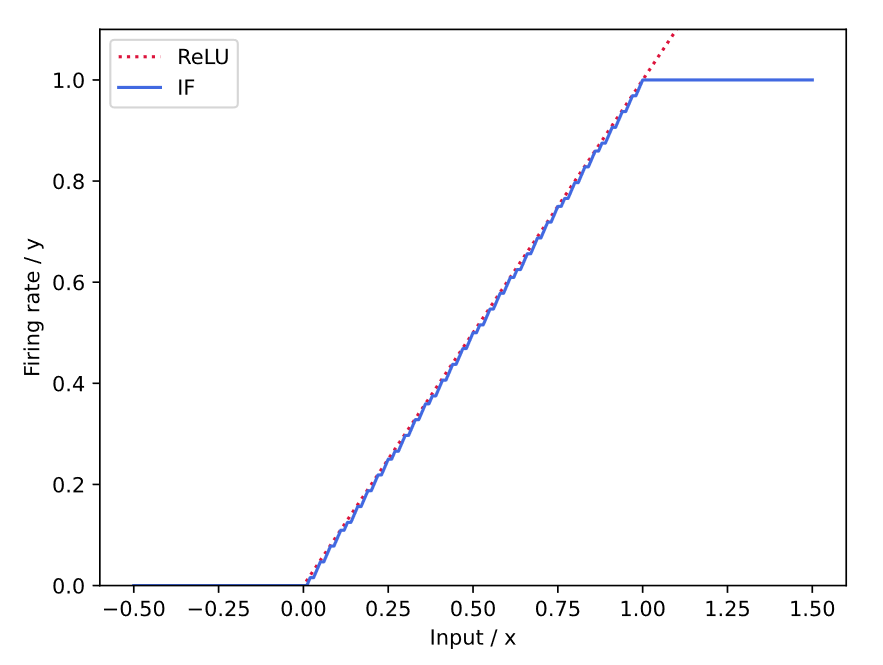
\includegraphics[width=0.4\textwidth]{as/fig2.png}
\caption{Firing rate of an IF neuron with soft reset compared with the output of a ReLU unit. Adapted from \autocite{liuHumanLevelControlDirectly2022}
}
\label{fig_2}
\end{figure}

\begin{figure}
\centering
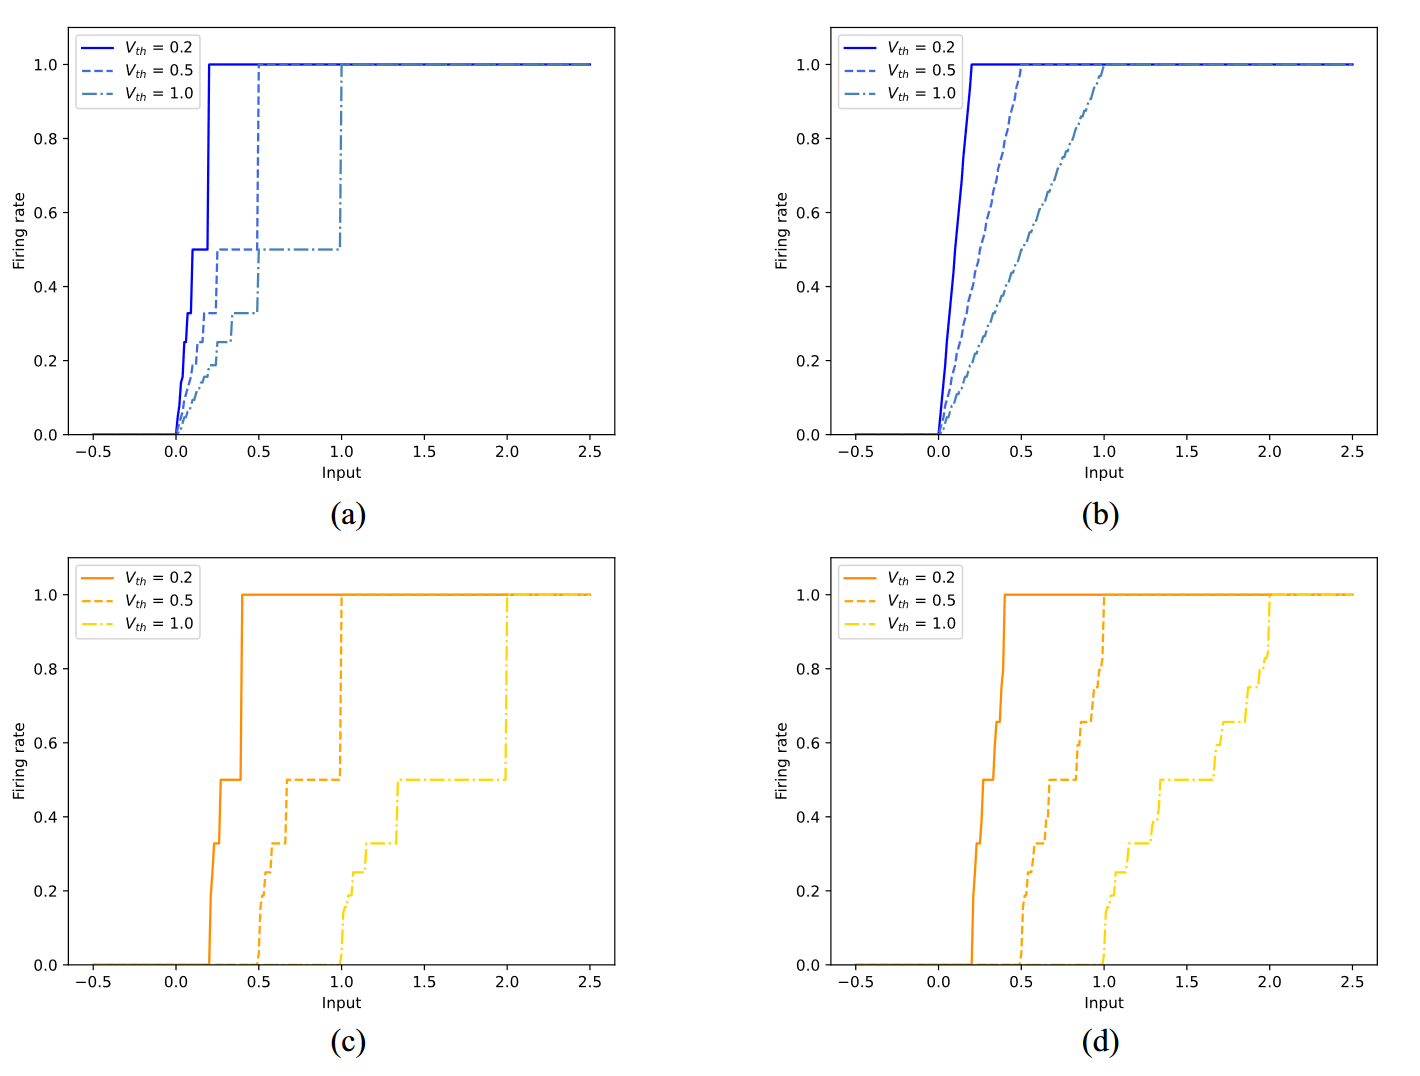
\includegraphics[width=0.6\textwidth]{as/fig3.png}
\caption{Comparisons between firing rate and inputs of the IF and LIF neurons in both hard and soft resets. \[V_{th}\] is set to 0.2, 0.5, and 1, respectively. \[V_{r} = 0\] constantly. (a) IF neuron reset by hard reset. (b) IF neuron reset by soft reset. (c) LIF neuron reset by hard reset. (d) LIF neuron reset by soft reset.  Adapted from \autocite{liuHumanLevelControlDirectly2022}
}
\label{fig_3}
\end{figure}

% \begin{figure*}[!t]
% \centering
% \subfloat{
% 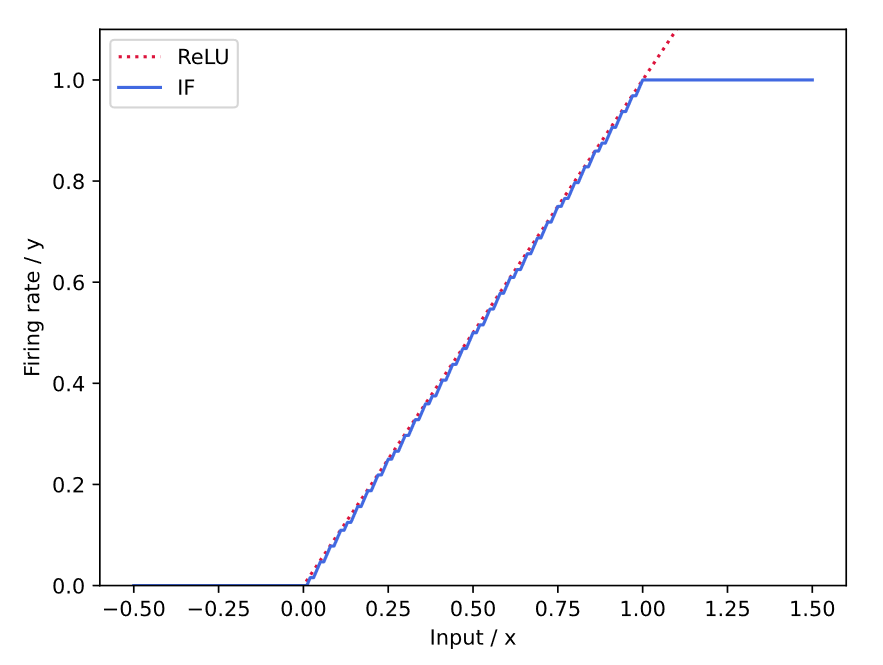
\includegraphics[width=3.5in]{as/fig2.png}%
% \label{fig_2}
% }
% \hfil
% \subfloat{
% 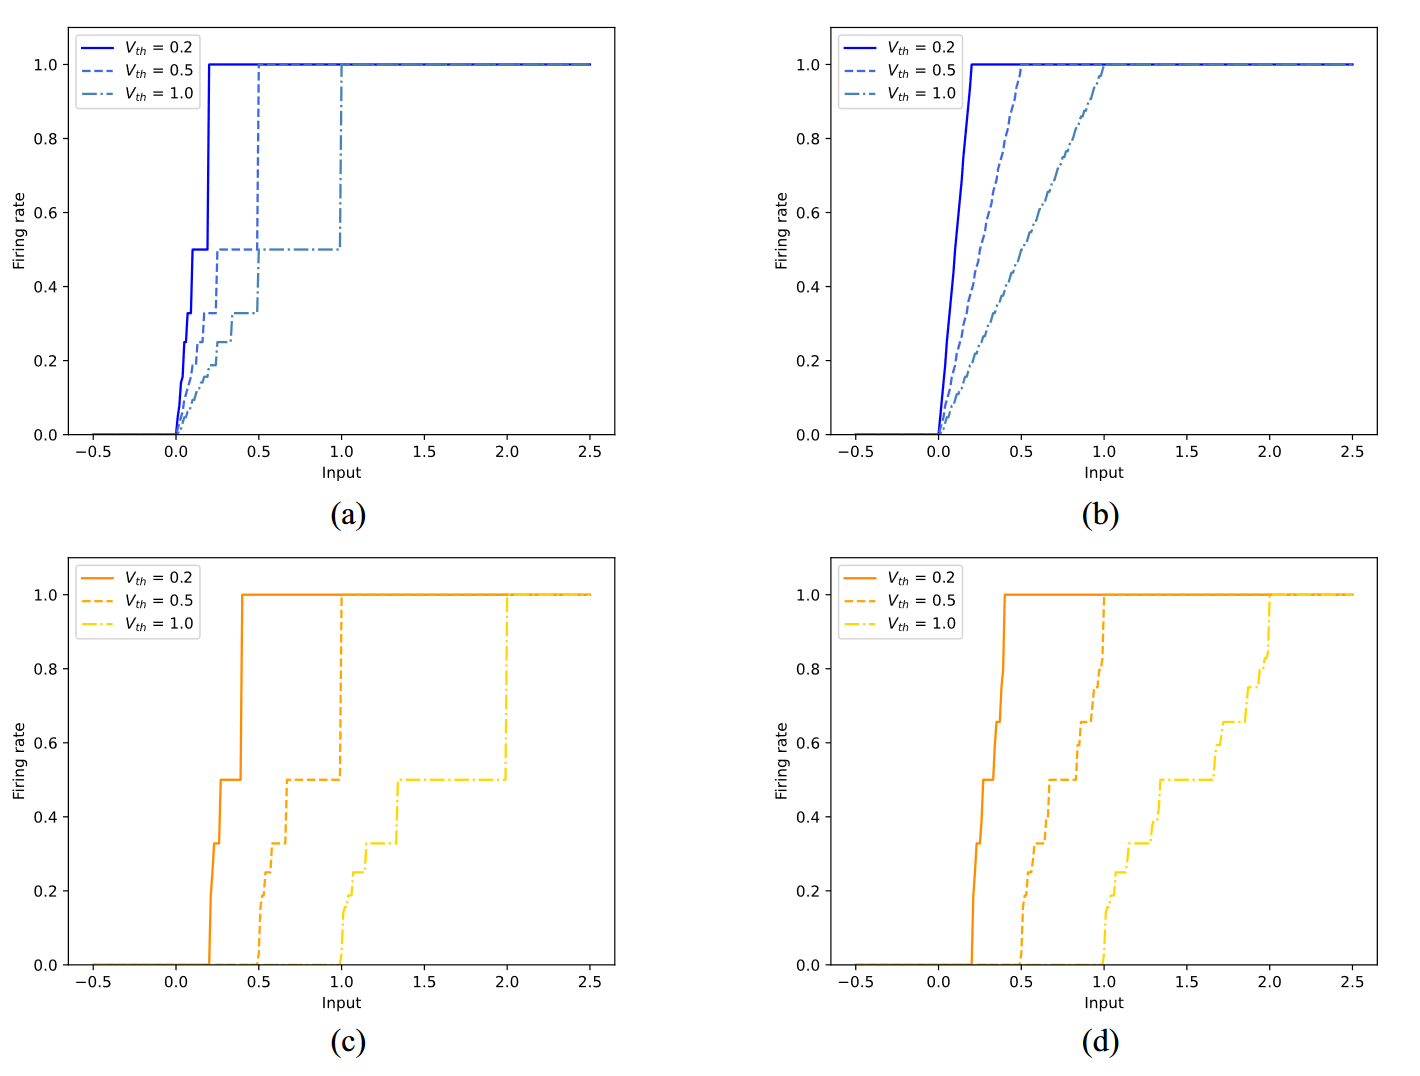
\includegraphics[width=3.5in]{as/fig3.png}%
% \label{fig_3}}
% \caption{Adapted from \autocite{liuHumanLevelControlDirectly2022}.
% }
% \label{fig_23}
% \end{figure*}


\section{Model Evaluation}\label{model-evaluation}

The qualities measured were performance, stability, learning
capability, and energy efficiency. They compared their results with
their own reproductions of the original DQN model in Mnih et al.~2015 as
well as the conversion-based SNN in Tan et al. 2020 \autocite{tanStrategyBenchmarkConverting2020}, using the 17 best
performing Atari games that were also used in Tan et al.~2020, these
are also the games for which the original DQN performed highest.

The in game frames are preprocessed to render them in grayscale and
down-resolutioned into 84 x 84 pixel images. The \(m\) most recent
frames (where \(m=4\)) are stacked as input. The real pixel values are
fed as input to the network without neural encoding.

The game is then simulated with a training time step occurring with a
window of 64 time steps for the DSQN and 100 time steps for the
conversion-based SNN.

In performance, of the 17 Atari games tested, the DSQN outperformed (in
terms of points) the DQN by an average of 106\%. The DSQN was able to
outperform the DQN on four games, scored equally in nine games, and
scored worst (maximum 20\% difference) in four of the games. The DSQN
proved to be more stable than the DQN, obtaining lower standard deviations in score in six games, equal to the DQN in two games, and inferior in nine games.

In learning capability, a total proof is not given. In Figure 4 the
learning curve for DQN and DSQN is compared for two games. From
these plots, it is apparent that the DSQN reaches a higher score
equilibrium faster than the DQN, as well as in the average max Q-value.
Though the authors claim this is representative in all cases, no metric
is provided. In the future an area under curve metric may be a useful
measure compare.

As with the DQN, we can see instability in the learning curves which is
native problem with the DQN. In DQNs this is mitigated through
implementation of a Double-DQN
\autocite{wengTianshouHighlyModularized2022} , where a
\emph{target network} is simultaneously trained to calculate the target
Q-values in the next state. The authors actually implement this DQN
model as well as the more recent CDQN
\autocite{wangConvergentEfficientDeep2022}. The authors claim
their implementations of these variations claim a better performance to
their ANN counterparts by 151.4\% and 141.8\% to the Double-DQN and CDQN
respectively. Unfortunately, no standard deviation measurements are
provided, but the comparison of Figure 4 and Figure 5 appears to
show less deviation.

Lastly, they score the model in terms of energy-efficiency. This is a
useful metric for prospective uses in neuromorphic hardware, where the
energy savings from spiking can be best obtained. However, there is no
direct method to compare the DSQN with the DQN in this manner. A rough estimate can be
made by comparing the number of calculations needed per inference. In
terms of energy transfer, the SNN must be evaluated in average spike
count. In this case, it was better to compare it to the conversion-based
SNN of \autocite{tanStrategyBenchmarkConverting2020}. The results show
the DSQN used around 85\% of the energy in comparison to the
conversion-based SNN. However, this comparison was only shown for two
games.

\begin{figure}
\centering
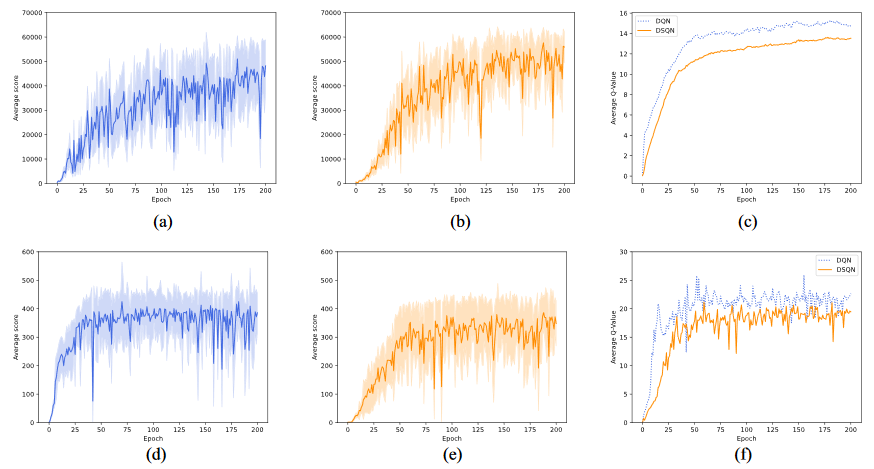
\includegraphics[width=0.7\textwidth]{as/fig4.png}
\caption{Learning curves of the DSQN and DQN in games Star Gunner and Breakout. Each episode is run for 30 rounds.(a), (b), (c), (d), and (e) plot the average score per episode. (c) and (f) plot the average max Q-value achieved per episode (epoch = 250,000 time steps). Adapted from \autocite{liuHumanLevelControlDirectly2022}.
}
\label{fig_4}
\end{figure}

\begin{figure}
\centering
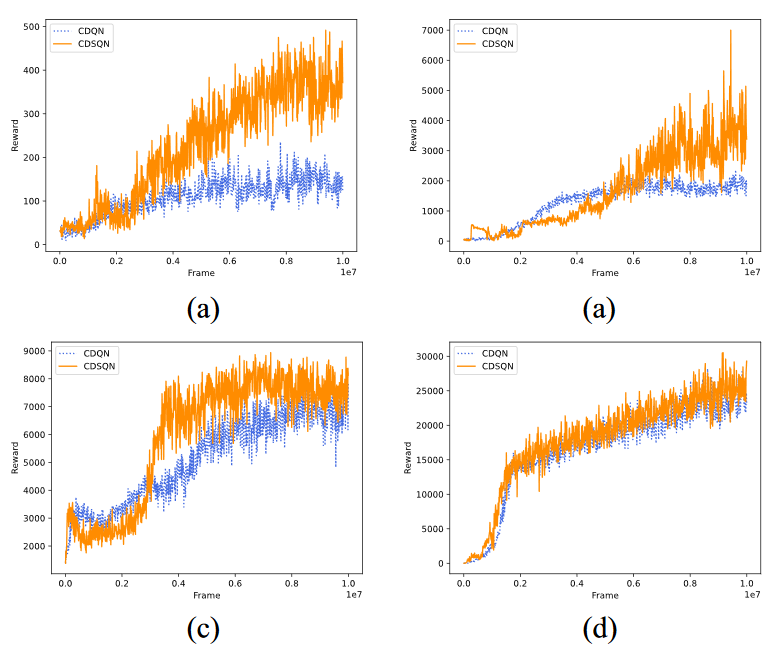
\includegraphics[width=0.7\textwidth]{as/fig5.png}
\caption{Learning curves of CDQN and CDSQN in four Atari games. Adapted from \autocite{liuHumanLevelControlDirectly2022}.
}
\label{fig_5}
\end{figure}

% \begin{figure*}[!t]
% \centering
% \subfloat[Case I]{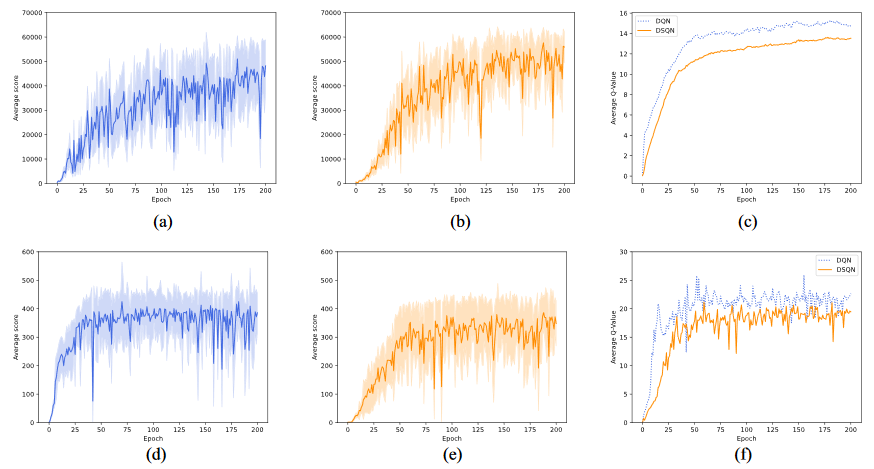
\includegraphics[width=2.5in]{as/fig4.png}%
% \label{fig_4}}
% \hfil
% \subfloat[Case II]{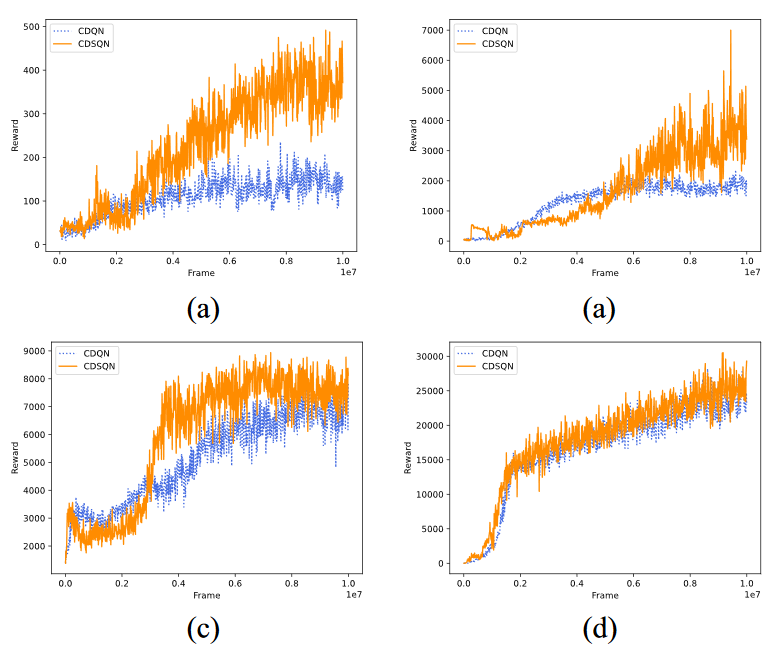
\includegraphics[width=2.5in]{as/fig5.png}%
% \label{fig_5}}
% \caption{Simulation results for the network.}
% \label{fig_sim}
% \end{figure*}

\section{Review}\label{review}

I find Liu et al.~2022 to be a very thorough and complete work which
takes the next logical step in deep reinforcement learning networks with
spiking neurons. This paper appears to be the first to showcase DRL in a
fully SNN model, as other models require conversion of pre-trained
ANNs, or mediatory ANN side-networks
\autocite{chenDeepReinforcementLearning2022}. The following
proof of increased performance and robustness with a full SNN model,
sets the stage for future models designed around total SNN architecture.

The paper is a very exhaustive with fine detail of network architecture,
neuron design, training methods, as well as thorough comparison with a
breadth of other models in the experiments. The provided methods and
code repositories makes readily the reproduction of their model. Though
as of writing, the original github repository is unavailable.

As with Mnih et al.~2015, this paper will likely serve as a benchmark for future DSRL models. The success of a fully spiking model in this example means development of further models which may
utilize SNN's efficiency to address problems with larger state and
action spaces.

Additionally, there are mechanisms here that future deep SNN learning
methods may be expected to duplicate. Namely, experience-replay, which
is again based on biological processes of memory formation and learning.
\autocite{mnihHumanlevelControlDeep2015} directly based the concept on
hippocampal replay wherein the during sleep, the brain replays
time-condensed activation of neural circuits associated with an
experienced physical activity
\autocite{bendorBiasingContentHippocampal2012}\autocite{oneillPlayItAgain2010}.
In SNNs, where spike timing larger oscillatory time cycles of neuron
activity known as phases are critical to network communication, perhaps
a designed neuronal circuit based around replicating the buffer like
memory and replaying the buffer in phases of time could be an aim of
future experiments.

Because the varieties of spiking neurons have no canonical set, further
experiments may be done with variations in neuron types, as well as
unique training methods specific to their mechanics. Testing the performance of spiking neuron varieties in a DSQN will provide a valuable point of comparison.

However, the reliance on gradient training may prove to be a
computational bottleneck. It may be prudent to then test the capacity
and computational costs of DSQNs. The unique properties of SNN
communication may lead to the development of alternative training techniques better suited to accelerate SNN performance.


\section{Future Directions}\label{furture-directions}

This paper marks an important milestone in the development of deep
spiking reward based models, but as an in-place model its efficacy in a naturalistic and dynamic environment, ones that RL and automata algorithms are typically designed for, is extremely limited. The experience-replay method effectively leverages a Q-learning
framework to work in a DNN, but this limits the DSQN model to an offline
training algorithm for an offline, single-task-specific network.

While not the totality of RL motivations, a reward based framework can
allow for a dynamically adapting model able to train in an online and
self-supervised environment. With the goal in mind of designing
autonomous and reactive hardware, there is a need for models which are
able to learn and adapt to unpredictable and isolated environments. The
DSQN can inform us of the capabilities of an in-place SNN trained with
an RL framework. The next step is to experiment with reward mechanisms
which will allow for dynamic learning in an online setting. To this end, it is necessary to replicate the abilities of SNNs similar to
those found in biological agents.

This problem is studied from the field of biologically inspired circuits is the \textit{spatial credit
assignment} problem. Similarly to RL, this problem of how to accurately assign reward, to neuronal circuits, which by nature are highly entangled and recurrent structures. and Local plasticity is a well-known mechanism of adaptation at
the neuron and neuronal assembly level. A well studied mechanism that is
being studied for use in SNNs is that of Spike-Timing Dependent
Plasticity (STDP) as well as its extension \emph{three-factor dependent
plasticity} which performs training updates on the basis of a
\emph{third-factor} which may come in the form of a reward-signal.
Additionally, plausible (though without biological basis) methods of back-propagation in SNNs have lately been proposed \autocite{payeurBurstdependentSynapticPlasticity2021}
\autocite{williamsNeuralBurstCodes2021} further adding alternative
plausible methods of credit-assignment in Deep-SNNs.

This however is a fairly nascent field, although emerging over two decades
ago in 1996 \autocite{maassNetworksSpikingNeurons1997}, it has gained
heavy traction in the past few years
\autocite{princeCurrentStateFuture2022}
\autocite{mehonicBraininspiredComputingNeeds2022} alongside
the acceleration of computational neuroscience and application-specific
integrated circuits in the machine learning space; and so there is a need
to develop and prove the efficacy of proposed methods in this space.

At this point, we are approaching a model of reinforcement learning from
an entirely new direction. This can be considered as a gap between
artificially driven methods and biologically-inspired ones, and there is
recent motivation to bridge the field of neuroscience back to deep
learning \autocite{zenkeVisualizingJointFuture2021} , by designing
entirely new mechanisms of reward-based learning that are effective in
SNNs, as opposed to attempting to apply the methods designed for ANNs,
then somewhat awkwardly fitting SNNs to them. This is not to say the
gains made from the ANN-to-SNN approach are non-contributing, but
instead we can use these proven models such as the DSQN to bridge the
gap from one direction and build towards it from the other. Any future
Deep SNN implementations will need to match the benchmark set here by
Liu et al.~2022.

% \hfill mds
 
% \hfill August 26, 2015

%\subsection{Subsection Heading Here}
%Subsection text here.

% needed in second column of first page if using \IEEEpubid
%\IEEEpubidadjcol

%\subsubsection{Subsubsection Heading Here}
%Subsubsection text here.


% An example of a floating figure using the graphicx package.
% Note that \label must occur AFTER (or within) \caption.
% For figures, \caption should occur after the \includegraphics.
% Note that IEEEtran v1.7 and later has special internal code that
% is designed to preserve the operation of \label within \caption
% even when the captionsoff option is in effect. However, because
% of issues like this, it may be the safest practice to put all your
% \label just after \caption rather than within \caption{}.
%
% Reminder: the "draftcls" or "draftclsnofoot", not "draft", class
% option should be used if it is desired that the figures are to be
% displayed while in draft mode.
%
%\begin{figure}[!t]
%\centering
%\includegraphics[width=2.5in]{myfigure}
% where an .eps filename suffix will be assumed under latex, 
% and a .pdf suffix will be assumed for pdflatex; or what has been declared
% via \DeclareGraphicsExtensions.
%\caption{Simulation results for the network.}
%\label{fig_sim}
%\end{figure}

% Note that the IEEE typically puts floats only at the top, even when this
% results in a large percentage of a column being occupied by floats.


% An example of a double column floating figure using two subfigures.
% (The subfig.sty package must be loaded for this to work.)
% The subfigure \label commands are set within each subfloat command,
% and the \label for the overall figure must come after \caption.
% \hfil is used as a separator to get equal spacing.
% Watch out that the combined width of all the subfigures on a 
% line do not exceed the text width or a line break will occur.
%
%\begin{figure*}[!t]
%\centering
%\subfloat[Case I]{\includegraphics[width=2.5in]{box}%
%\label{fig_first_case}}
%\hfil
%\subfloat[Case II]{\includegraphics[width=2.5in]{box}%
%\label{fig_second_case}}
%\caption{Simulation results for the network.}
%\label{fig_sim}
%\end{figure*}
%
% Note that often IEEE papers with subfigures do not employ subfigure
% captions (using the optional argument to \subfloat[]), but instead will
% reference/describe all of them (a), (b), etc., within the main caption.
% Be aware that for subfig.sty to generate the (a), (b), etc., subfigure
% labels, the optional argument to \subfloat must be present. If a
% subcaption is not desired, just leave its contents blank,
% e.g., \subfloat[].


% An example of a floating table. Note that, for IEEE style tables, the
% \caption command should come BEFORE the table and, given that table
% captions serve much like titles, are usually capitalized except for words
% such as a, an, and, as, at, but, by, for, in, nor, of, on, or, the, to
% and up, which are usually not capitalized unless they are the first or
% last word of the caption. Table text will default to \footnotesize as
% the IEEE normally uses this smaller font for tables.
% The \label must come after \caption as always.
%
%\begin{table}[!t]
%% increase table row spacing, adjust to taste
%\renewcommand{\arraystretch}{1.3}
% if using array.sty, it might be a good idea to tweak the value of
% \extrarowheight as needed to properly center the text within the cells
%\caption{An Example of a Table}
%\label{table_example}
%\centering
%% Some packages, such as MDW tools, offer better commands for making tables
%% than the plain LaTeX2e tabular which is used here.
%\begin{tabular}{|c||c|}
%\hline
%One & Two\\
%\hline
%Three & Four\\
%\hline
%\end{tabular}
%\end{table}


% Note that the IEEE does not put floats in the very first column
% - or typically anywhere on the first page for that matter. Also,
% in-text middle ("here") positioning is typically not used, but it
% is allowed and encouraged for Computer Society conferences (but
% not Computer Society journals). Most IEEE journals/conferences use
% top floats exclusively. 
% Note that, LaTeX2e, unlike IEEE journals/conferences, places
% footnotes above bottom floats. This can be corrected via the
% \fnbelowfloat command of the stfloats package.




% \section{Conclusion}
% The conclusion goes here.





% if have a single appendix:
%\appendix[Proof of the Zonklar Equations]
% or
%\appendix  % for no appendix heading
% do not use \section anymore after \appendix, only \section*
% is possibly needed

% use appendices with more than one appendix
% then use \section to start each appendix
% you must declare a \section before using any
% \subsection or using \label (\appendices by itself
% starts a section numbered zero.)
%


% \appendices
% \section{Proof of the First Zonklar Equation}
% Appendix one text goes here.

% you can choose not to have a title for an appendix
% if you want by leaving the argument blank
% \section{}
% Appendix two text goes here.


% % use section* for acknowledgment
% \section*{Acknowledgment}


% The authors would like to thank...


% Can use something like this to put references on a page
% by themselves when using endfloat and the captionsoff option.
\ifCLASSOPTIONcaptionsoff
  \newpage
\fi



% trigger a \newpage just before the given reference
% number - used to balance the columns on the last page
% adjust value as needed - may need to be readjusted if
% the document is modified later
%\IEEEtriggeratref{8}
% The "triggered" command can be changed if desired:
%\IEEEtriggercmd{\enlargethispage{-5in}}

% references section
\newpage
% can use a bibliography generated by BibTeX as a .bbl file
% BibTeX documentation can be easily obtained at:
% http://mirror.ctan.org/biblio/bibtex/contrib/doc/
% The IEEEtran BibTeX style support page is at:
% http://www.michaelshell.org/tex/ieeetran/bibtex/
%\bibliographystyle{IEEEtran}
% argument is your BibTeX string definitions and bibliography database(s)
%\bibliography{IEEEabrv,../bib/paper}
%
% <OR> manually copy in the resultant .bbl file
% set second argument of \begin to the number of references
% (used to reserve space for the reference number labels box)
%\begin{thebibliography}{1}
% \printbibliography[heading = bibintoc, title = Bibliography]   
\printbibliography[] 
% \bibitem{IEEEhowto:kopka}
% H.~Kopka and P.~W. Daly, \emph{A Guide to \LaTeX}, 3rd~ed.\hskip 1em plus
%   0.5em minus 0.4em\relax Harlow, England: Addison-Wesley, 1999.

%\end{thebibliography}

% biography section
% 
% If you have an EPS/PDF photo (graphicx package needed) extra braces are
% needed around the contents of the optional argument to biography to prevent
% the LaTeX parser from getting confused when it sees the complicated
% \includegraphics command within an optional argument. (You could create
% your own custom macro containing the \includegraphics command to make things
% simpler here.)
%\begin{IEEEbiography}[{\includegraphics[width=1in,height=1.25in,clip,keepaspectratio]{mshell}}]{Michael Shell}
% or if you just want to reserve a space for a photo:

% \begin{IEEEbiography}{Michael Shell}
% Biography text here.
% \end{IEEEbiography}

% % if you will not have a photo at all:
% \begin{IEEEbiographynophoto}{John Doe}
% Biography text here.
% \end{IEEEbiographynophoto}

% % insert where needed to balance the two columns on the last page with
% % biographies
% %\newpage

% \begin{IEEEbiographynophoto}{Jane Doe}
% Biography text here.
% \end{IEEEbiographynophoto}

% You can push biographies down or up by placing
% a \vfill before or after them. The appropriate
% use of \vfill depends on what kind of text is
% on the last page and whether or not the columns
% are being equalized.

%\vfill

% Can be used to pull up biographies so that the bottom of the last one
% is flush with the other column.
%\enlargethispage{-5in}



% that's all folks
\end{document}